\section{Homotopy between maps, homotopy as equivalence relation, path homotopy}

\begin{example}
    \( \mathbb{S}^1 \) is compact, but \( \mathbb{R} \) is not.
    So \( \mathbb{S}^1 \not\simeq \mathbb{R} \).
\end{example}

\begin{example}
    \( \mathbb{R} \setminus \{ p \}  \) is not connected.
    Assume that there exists a homeomorphism
    \[
      f: \mathbb{R} \to \mathbb{R}^2
    \]
    \( f \) induces a map
    \[
      \hat{f}: \mathbb{R} \setminus \{ p \}  \to \mathbb{R}^2 \setminus \{ f(p) \} 
    \]
    but \( \mathbb{R}^2 \setminus \{ f(p) \}  \) is connected.
    Hence \( \mathbb{R} \not\simeq \mathbb{R}^2 \).
\end{example}

Denote by \( I \) the closed interval \( [0, 1] \subseteq \mathbb{R} \)
with the usual topology.

\subsection{Homotopy theory}

\subsection{Homotopies}

\begin{definition}[Homotopy]
    Let \( f,g: X \to Y \) be continuous maps
    of topological spaces.
    We say that \( f \) is homotopic to \( g \)
    if there exists a continuous map
    \( H: I \times X \to Y \) such that
    \begin{align}
      H(0, x) &= f(x) \\
      H(1, x) &= g(x)
    \end{align}
    We denote that two maps \( f \) and \( g \) are homotopic
    by writing \( f \simeq g \).
\end{definition}

\begin{definition}[Nullhomotopy]
   A continuous map \( f: X \to Y \)
   is nullhomotopic if it is homotopic
   to a constant map.
\end{definition}

\begin{example}
    Consider two maps \( f, g: X \to \mathbb{R}^n \).
    They are homopotic via the homotopy
    \begin{equation}
        H(t, x) = (1-t) f(x) + t g(x)
    \end{equation}
    Now, \( H \) is continuous, and Fernando says:
    \begin{displayquote}
      If this is not continuous, life has no purpose.
    \end{displayquote}
    To see that \( H \) is continous, consider the following
    diagrams and argue by composition of known continous maps:
    % https://q.uiver.app/#q=WzAsNixbMCwwLCJJIFxcdGltZXMgWCJdLFsyLDAsIlxcbWF0aGJie1J9Xm4gXFx0aW1lcyBcXG1hdGhiYntSfV5uIl0sWzQsMCwiXFxtYXRoYmJ7Un1ebiJdLFswLDEsIih0LHgpIl0sWzIsMSwiKCgxLXQpZih4KSx0Zyh4KSkiXSxbNCwxLCIoMS10KWYoeCkgKyB0Zyh4KSJdLFswLDEsIlxcZ2FtbWFcXHRpbWVzXFx2YXJwaGkiXSxbMSwyLCJcXG9wbHVzIl0sWzMsNF0sWzQsNV1d
\[\begin{tikzcd}
	{I \times X} && {\mathbb{R}^n \times \mathbb{R}^n} && {\mathbb{R}^n} \\
	{(t,x)} && {((1-t)f(x),tg(x))} && {(1-t)f(x) + tg(x)}
	\arrow["{\gamma\times\varphi}", from=1-1, to=1-3]
	\arrow["\oplus", from=1-3, to=1-5]
	\arrow[from=2-1, to=2-3]
	\arrow[from=2-3, to=2-5]
\end{tikzcd}\]
where \( \gamma \) and \( \varphi \) are defined by
% https://q.uiver.app/#q=WzAsNyxbMSwwLCJJIFxcdGltZXMgWCJdLFszLDAsIlxcbWF0aGJie1J9IFxcdGltZXMgXFxtYXRoYmJ7Un1ebiJdLFs1LDAsIlxcbWF0aGJie1J9Xm4iXSxbMSwxLCIodCx4KSJdLFszLDEsIih0LGcoeCkpIl0sWzUsMSwidGcoeCkiXSxbMCwwLCJcXHZhcnBoaToiXSxbMCwxLCJcXHRleHR7aWR9XFx0aW1lcyBnIl0sWzEsMl0sWzMsNF0sWzQsNV1d
\[\begin{tikzcd}
	{\varphi:} & {I \times X} && {\mathbb{R} \times \mathbb{R}^n} && {\mathbb{R}^n} \\
	& {(t,x)} && {(t,g(x))} && {tg(x)}
	\arrow["{\text{id}\times g}", from=1-2, to=1-4]
	\arrow[from=1-4, to=1-6]
	\arrow[from=2-2, to=2-4]
	\arrow[from=2-4, to=2-6]
\end{tikzcd}\]
% https://q.uiver.app/#q=WzAsNyxbMSwwLCJJIFxcdGltZXMgWCJdLFszLDAsIlxcbWF0aGJie1J9IFxcdGltZXMgXFxtYXRoYmJ7Un1ebiJdLFs1LDAsIlxcbWF0aGJie1J9Xm4iXSxbMSwxLCIodCx4KSJdLFszLDEsIih0LGYoeCkpIl0sWzUsMSwiKDEtdClmKHgpIl0sWzAsMCwiXFxnYW1tYToiXSxbMCwxLCJcXHRleHR7aWR9XFx0aW1lcyBmIl0sWzEsMl0sWzMsNF0sWzQsNV1d
\[\begin{tikzcd}
	{\gamma:} & {I \times X} && {\mathbb{R} \times \mathbb{R}^n} && {\mathbb{R}^n} \\
	& {(t,x)} && {(t,f(x))} && {(1-t)f(x)}
	\arrow["{\text{id}\times f}", from=1-2, to=1-4]
	\arrow[from=1-4, to=1-6]
	\arrow[from=2-2, to=2-4]
	\arrow[from=2-4, to=2-6]
\end{tikzcd}\]
From this we conclude that any
two maps with target in \( \mathbb{R}^n \)
are homotopic. In particular, every
map is nullhomotopic.
\end{example}

\begin{definition}
    Let \( X, Y \) be topological spaces.
    Define
    \begin{equation}
      \hom_{\text{Top}}(X, Y) = \{ f:X \to Y \mid f \text{cont.} \} 
    \end{equation}
\end{definition}

\begin{lemma}[Pasting lemma]
   Let \( X = A \cup B \) be a topological space
   where \( A, B \) are closed subsets.
   Suppose  \( f: A \to Y \) and \( g: B \to Y \) are
   continuous maps such that
  \[
    f|_{A\cap B} = g|_{A\cap B}.
  \] 
  Then there exists a continuous map \( h:X \to Y \)
  such that
  \[
    h|_A = f, h|_B = g.
  \]
\end{lemma}

\begin{proof}
    Define \( h:X \to Y \) by
    \[
      h(x) = \begin{cases}
        f(x) & x \in A \\
        g(x) & x \in B
      \end{cases}
    \]
    \( h \) is well defined since \( f \) and \( g \) agree
    on the intersection of \( A \) and \( B \).
    Take a closed subset \( Z \subseteq Y \).
    Then
    \begin{align*}
      {h}^{-1} (Z) &=( {h}^{-1} (Z) \cap A ) \cup ( {h}^{-1} (Z) \cap B ) \\
                   &= {f}^{-1} (Z) \cup {g}^{-1} (Z)
    \end{align*}
    And since \( f, g \) are cont. and \( Z \) closed
    we get that \( {f}^{-1} (Z) \subseteq A \subseteq X \)
    and \( {g}^{-1} (Z) \subseteq B \subseteq X \) are closed.
    Furthermore, a finite union of closed subsets is closed,
    so \( {h}^{-1} (Z) \) is closed.
\end{proof}

\begin{theorem}
   Homotopies are an equivalence relation on  \( \hom_{\text{Top}}(X, Y) \) .
\end{theorem}

\begin{proof} We prove reflexivity, symmetry and transitivity.
    \begin{enumerate}
      \item[1)] Define \( H: I \times X \to X \) by sending
        \( (t, x) \) to \( f(x) \).
        Then \( H(0, x) = H(1,x) = f(x) \).
      \item[2)] Let \( H \) be a homotopy of \( f \) and \( g \).
        Define \( \overline{H} \) by
% https://q.uiver.app/#q=WzAsNixbMSwwLCJJIFxcdGltZXMgWCJdLFszLDAsIkkgXFx0aW1lcyBYIl0sWzUsMCwiWSJdLFsxLDEsIih0LCB4KSJdLFszLDEsIigxLXQsIHgpIl0sWzAsMCwiXFxvdmVybGluZXtIfToiXSxbMCwxXSxbMSwyLCJIIl0sWzMsNF1d
\[\begin{tikzcd}
	{\overline{H}:} & {I \times X} && {I \times X} && Y \\
	& {(t, x)} && {(1-t, x)}
	\arrow[from=1-2, to=1-4]
	\arrow["H", from=1-4, to=1-6]
	\arrow[from=2-2, to=2-4]
\end{tikzcd}\]
Then it is easy to see that \( g \simeq f \).
      \item[3)] Let \( H_1 \) and \( H_2 \) be homotopies
        for \( f \simeq g \) and \( g \simeq h \) respectivly.
        Define
        \begin{equation}
            H_3(t, x) = \begin{cases}
              H_1(2t, x) & 0 \le t \le 1/2 \\
              H_2(2t-1, x) & 1/2 \le t \le 1
            \end{cases}
        \end{equation}
        \( H_3 \) is continuous by the pasting lemma.
        It is easy to check that it is a homotopy.
    \end{enumerate}
\end{proof}

\begin{definition}
    Notation:
    \begin{align}
      [X, Y] &= \hom_{\text{Top}} ( X, Y) / \simeq \\
      [f] &= \{ g: X \to Y \mid f \simeq g, g \in \hom_{\text{Top}} ( X, Y) \}
    \end{align}
\end{definition}

\begin{definition}
    Denote by \( * \) the singelton set.
    \begin{equation}
      [*, Y] = Y / (y_0 \sim y_1 \text{if a path exists}) = \pi_0(Y)
    \end{equation}
\end{definition}

\( Y \) path connected \( \iff \) \( \pi_0(Y) = * \).

\subsection{Path homotopies}

\begin{definition}[Path homotopy]
   Let \( f,g: I \to X \) be paths from
   \( x_0 \) to \( x_1 \).
    We say that \( f \) is path homotopic
    to \( g \) and write \( f \simeq_{p} g \) if
    there exists a continuous function
    \( H: I \times I \to X \) such that
    \begin{align*}
      H(0, s) = f(s)&, H(1, s) = g(s) \\
      H(t, 0) = x_0&, H(t, 1) = x_1
    \end{align*}
\end{definition}

\begin{example}
    Let \( D^2 = \{ (x, y) \in \mathbb{R}^2 \} \mid x^2 + y^2 \le 1  \)
    be the unit disk. Consider \( D^2 \setminus \{ (0, 0) \}  \).
    Then \( f \not\simeq_p g \).
    \begin{center}
      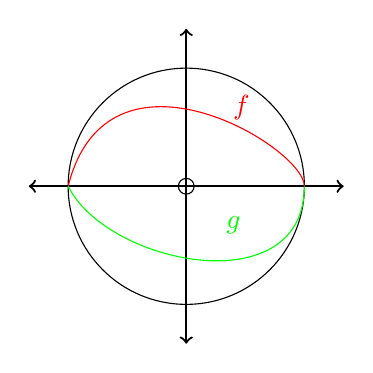
\begin{tikzpicture}
        \draw[thick, <->] (-2, 0)  -- (2, 0);
        \draw[thick, <->] (0, -2)  -- (0, 2);

        \draw (0, 0) circle (1.5);
        \draw (0, 0) circle (0.1);

        \draw[red] (-1.5, 0) .. controls (-1, 2) and (1.5, 0.5) .. (1.5, 0) node at (0.7,1) {\( f \)};
        \draw[green] (-1.5, 0) .. controls (-1, -1) and (1.5, -1.5) .. (1.5, 0) node at (0.6, -0.5) {\( g \)};
      \end{tikzpicture}
    \end{center}
\end{example}

\begin{definition}
  \( \hom_{\text{Top}}^{x_0, x_1} = \{ f: I \to X \mid f \text{cont.}, f(0) = x_0, f(1) = x_1  \}  \).
\end{definition}

\begin{theorem}
    Path homotopies define an equivalence relation on \( \hom_{\text{Top}}^{x_0, x_1} \).
\end{theorem}

\begin{proof}
    Similar as the proof of homotopy equivalence relation.
\end{proof}
